\section{LDA Ensemble for Face Recognition}
\label{sec:intro}

PCA can effectively reduce the dimension of input data preserving important features. And LDA can maximize the variance of between-class while minimize between-class. Thus, using PCA-LDA is expected to increase computing efficiency and classification accuracy. In this section, we try to figure out the effect of PCA-LDA via some experiments.

%-------------------------------------------------------------------------
\subsection{Recognition accuracy of PCA-LDA}

To implement PCA-LDA, we set $M_{pca}$ and $M_{lda}$ by measuring classification accuracy with $M_{pca}$ from 1 to 415 and $M_{lda}$ from 1 to $min(M_{pca}-1, 51)$. This is because, the maximum possible projection dimension for PCA is $N-1$ since the total number of principal components can not be larger than overall data, and for LDA is $n_{class}-1$ since the number of direction for maximizing the distance of between-class and minimizing within-class cannot be larger than the total number of classes. As shown in \cref{fig:mpca_mlda}, accuracy peaked at $M_{pca}=150$ and $M_{lda}=50$. Higher $M_{lda}$ improves performance by enhancing data discrimination, while optimal $M_{pca}$ is between 100 and 200, balancing information retention and overfitting risk.


In LDA, the rank of within-class scatter matrix($S_w$) is $min(364, M_{pca})$, where $N-n_{class}=416-52=364$ and the rank of between-class scatter matrix($S_b$) is $n_{class}-1=51$. Since $\sum_{x\in D_i} (x-m_i) = 0$, each class is linearly dependent, so, $S_w = \sum_{i=1}^c \sum_{x\in D_i} (x-m_i)(x-m_i)^T$ has at most $N-n_{class}$ linearly independent row vectors. After reducing dimensions using PCA, the rank of $S_w$ cannot exceed $M_{pca}$ as the vectors are confined to the PCA subspace. For $S_b$ defined as $S_b = \sum_{i=1}^c (m_i-m)(m_i-m)^T$, it depends only ionly on class means, and since their relationship of class mean does not change after PCA projection since their relationships remain unchanged under PCA (a linear transformation), the maximum possible rank for $S_b$ is $N - n_{class}$.

Based on this observation, we decided to fix $M_{pca}=150$ and $M_{lda}=50$ for further experiments. 

\begin{figure}
  \centering
   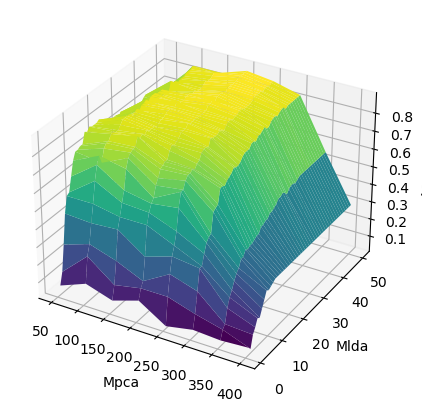
\includegraphics[width=0.8\linewidth]{image/mpca_mlda.png}

   \caption{Classification accuracy varying Mpca and Mlda}
   \label{fig:mpca_mlda}
\end{figure}


%-------------------------------------------------------------------------
\subsection{Result of PCA-LDA}

\cref{fig:q3_1_cm} is the confusion matrix of PCA-LDA classification result. As most of prediction result is on the diagonal entry, it indicates that most of prediction is successful. We take a closer look at success and failure cases. \cref{fig:q3_success} shows successfully predicted cases. Despite the different angles of the faces, the model infer the class accurately. \cref{fig:q3_fail} is failure cases. It seems that the prediction failed because of the similar glasses and face expression.


% %-------------------------------------------------------------------------
% \subsection{Time and Memory}
% Comparison btw pca/pca-lda (accuracy), lda/pca-lda(time), pca/lda/pca-lda(memory)

% %-------------------------------------------------------------------------
% \subsection{PCA-LDA Ensemble}
% For PCA-LDA Ensemble model, we combined two different types of models. The first type is randomization in feature space, which select vectors for pca projection randomly by a certain percentage. The second type is randomization in data sampling, which randomly subsampling the train data by a certain percentage. Both models were used in equal numbers. For combining prediction results of each models, we used 'majority voting' among various fusion rules. This is because, since our task is predicting class for classification and each classes don't have special meaning in numeric value, majority voting looks the most reasonable compared to other methods like averaging and finding maximum. 

%-------------------------------------------------------------------------
\subsection{PCA-LDA Ensemble}
% randomization in feature space (m0)
% randomization in data samples (subset\_rate)
% randomization in model number (model\_num)
% randomness parameter

There are 3 hyperparameter that we can handle randomness: the number of random vector in feature space, the proportion of training data for subsampling, and the number of models for the ensemble. We will examine the impact of each one one by one.

\begin{figure}
	\centering
	\begin{subfigure}[t]{0.48\linewidth}
		\centering
		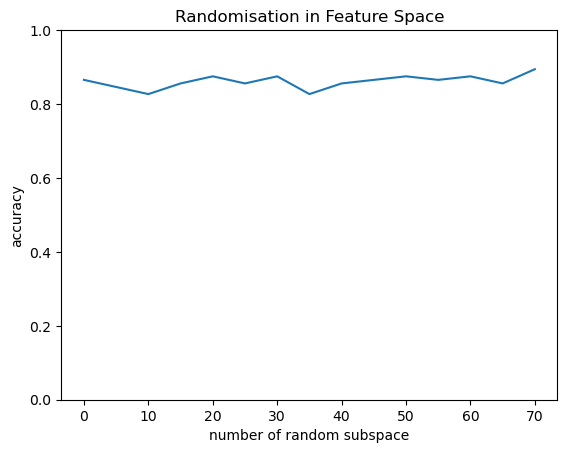
\includegraphics[width=\linewidth]{image/q3_fs_rs.png}
		\caption{Randomization in feature space}
		\label{fig:q3_fs}
	\end{subfigure}%
	\hfill
	\begin{subfigure}[t]{0.48\linewidth}
		\centering
		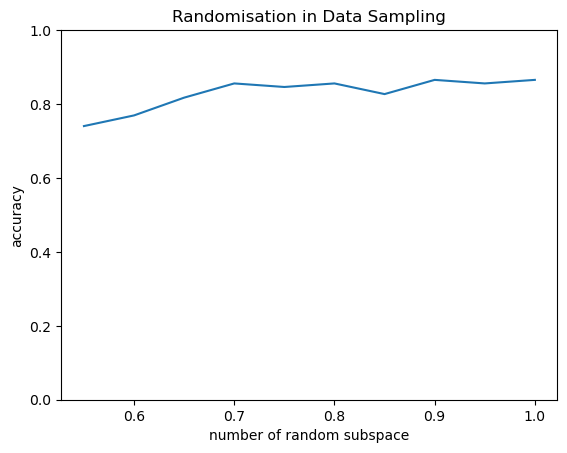
\includegraphics[width=\linewidth]{image/q3_data_rs.png}
		\caption{Random data subsamplint}
		\label{fig:q3_data}
	\end{subfigure}
	
	\begin{subfigure}[t]{0.48\linewidth}
		\centering
		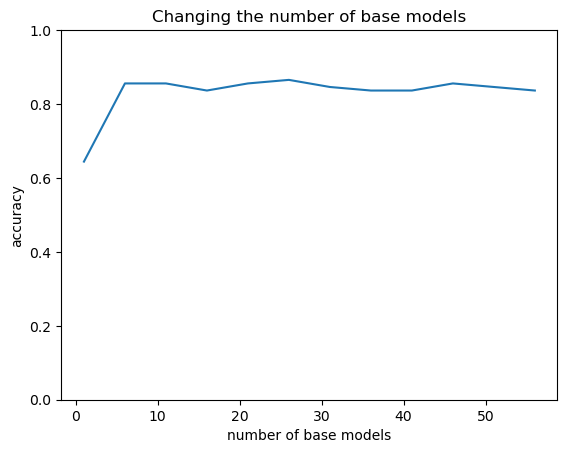
\includegraphics[width=\linewidth]{image/q3_basemodel.png}
		\caption{randomization in the number of basemodels}
		\label{fig:q3_base}
	\end{subfigure}
	\caption{Accuracy comparison between randomness parameters}
	\label{fig:q3_random}
\end{figure}

First, we look into randomization in feature space($M1$). As \cref{fig:q3_fs} indicates, the accuracy is almost highest when the number of random samples is around 30. This is because if the number of random vectors is too large, important features cannot be preserved, and if it is too small, overfitting occurs. Therefore, it is estimated that optimization occurred when the number of random vectors was 30.

Next, we observe the impact of data subsampling proportion($\alpha$). \cref{fig:q3_data} shows the accuracy with respect to the proportion of sub-sampled data. The more data we use, the better accuracy we get. This is quite predictable since the more data you have, the easier it is to generalize.

Lastly, regarding the effect of the number of base models($n_{model}$), we varied the number from 1 to 60, as shown in \cref{fig:q3_base}. When there are fewer than 30 models, the results are similar to a single PCA-LDA model. However, with more than 30 models, performance improves significantly, though further increases beyond 30 yield minimal gains. This is because up to 30 models, the ensemble can capture diverse features for generalization, but the PCA-LDA model’s limited ability to capture complex patterns prevents substantial improvement beyond that point. We used "majority voting" for combining predictions, as it’s most suitable for classification tasks where each class lacks numeric meaning, making it more appropriate than methods like averaging or maximum selection.

Considering both accuracy and computation cost, we conclude that the ensemble model with $M1=30$, $\alpha=0.9$, $n_{model}=30$ has the best performance.

% randomness parameter?

%-------------------------------------------------------------------------
\subsection{Result of PCA-LDA Ensemble}
The accuracy of committee machine, which gather all prediction results from each base models from ensemble model, is 0.846. And the average of individual models in ensemble model is 0.736. From this result, we can check that the performance of committee machine is better than individual as we learned. (Ensemble Learning LN, p.11-13)

In addition, \cref{fig:q3_2_cm} shows the confusion matrix of ensemble model. Compared to \cref{fig:q3_1_cm}, since \cref{fig:q3_2_cm} has less components outside the diagonal, we can visually check that the accuracy of classification of ensemble model is higher than single PCA-LDA model.
